\documentclass[11pt]{article}
\usepackage{epsfig,psfrag}
\usepackage{amsmath}

\setlength{\textwidth}{6.2in}
\setlength{\oddsidemargin}{0.3in}
\setlength{\evensidemargin}{0in}
\setlength{\textheight}{8.7in}
\setlength{\voffset}{-.7in}
\setlength{\headsep}{26pt}
\setlength{\parindent}{10pt}
\begin{document}


% a few handy macros

\newcommand\matlab{{\sc matlab}}
\newcommand{\goto}{\rightarrow}
\newcommand{\bigo}{{\mathcal O}}
\newcommand{\half}{\frac{1}{2}}
%\newcommand\implies{\quad\Longrightarrow\quad}
\newcommand\reals{{{\rm l} \kern -.15em {\rm R} }}
\newcommand\complex{{\raisebox{.043ex}{\rule{0.07em}{1.56ex}} \hskip -.35em {\rm C}}}


% macros for matrices/vectors:

% matrix environment for vectors or matrices where elements are centered
\newenvironment{mat}{\left[\begin{array}{ccccccccccccccc}}{\end{array}\right]}
\newcommand\bcm{\begin{mat}}
\newcommand\ecm{\end{mat}}

% matrix environment for vectors or matrices where elements are right justifvied
\newenvironment{rmat}{\left[\begin{array}{rrrrrrrrrrrrr}}{\end{array}\right]}
\newcommand\brm{\begin{rmat}}
\newcommand\erm{\end{rmat}}

% for left brace and a set of choices
\newenvironment{choices}{\left\{ \begin{array}{ll}}{\end{array}\right.}
\newcommand\when{&\text{if~}}
\newcommand\otherwise{&\text{otherwise}}
% sample usage:
%  \delta_{ij} = \begin{choices} 1 \when i=j, \\ 0 \otherwise \end{choices}


% for labeling and referencing equations:
\newcommand{\eql}{\begin{equation}\label}
\newcommand{\eqn}[1]{(\ref{#1})}
% can then do
%  \eql{eqnlabel}
%  ...
%  \end{equation}
% and refer to it as equation \eqn{eqnlabel}.  


% some useful macros for finite difference methods:
\newcommand\unp{U^{n+1}}
\newcommand\unm{U^{n-1}}

% for chemical reactions:
\newcommand{\react}[1]{\stackrel{K_{#1}}{\rightarrow}}
\newcommand{\reactb}[2]{\stackrel{K_{#1}}{~\stackrel{\rightleftharpoons}
   {\scriptstyle K_{#2}}}~}

  % input some useful macros

% Macros for exercises:

\newcommand{\exernum}{0.0} % will be set to current Exercise number

% Headers:

\newcommand{\exercise}[2][\null]{\vskip 15pt \noindent%
     {\large \bf Exercise #2}~ {\it #1}%
     \nopagebreak\vskip 5pt \nopagebreak%
     \renewcommand{\exernum}{#2} \setcounter{equation}{0}%
     \addcontentsline{toc}{subsection}{Exercise #2 \hskip 5pt #1}}
     % \exercise has optional first argument -- short descriptor
     % the exercise number is stored in \exernum for use in labeling equations

\newcommand{\chapexercises}[1]{%
     \cleardoublepage
     \centerline{\LARGE\bf Chapter #1 Exercises}
     \vskip .5cm
     \noindent
     From: {\it Finite Difference Methods for Ordinary and Partial 
     Differential Equations}\\  by R.~J.~LeVeque, SIAM, 2007.~~~
     {\tt http://www.amath.washington.edu/$\sim$rjl/fdmbook}
     \vskip .5cm
     \addcontentsline{toc}{section}{Chapter #1}
     }

% Parts:

% set enumerate to give parts a, b, c, ...  rather than numbers 1, 2, 3...
\renewcommand{\theenumi}{\alph{enumi}}
\renewcommand{\labelenumi}{(\theenumi)}

% set second level enumerate to give parts i, ii, iii, iv, etc.
\renewcommand{\theenumii}{\roman{enumii}}
\renewcommand{\labelenumii}{(\theenumii)}

% Equations:

% label equations starting with E for exercise, then exernum, then a,b,c etc
\renewcommand{\theequation}{Ex\exernum\alph{equation}}


% commands for labeling and citing equations to add exernum automatically.
%   then set equations using e.g. \eqlex{a} ... \end{equation}
%   and cite as \eqnex{a}
\newcommand{\eqlex}[1]{\begin{equation}\label{\exernum #1}}
\newcommand{\eqnex}[1]{(\ref{\exernum #1})}
       % more macros for exercise formatting

% For exercises,
% set enumerate to give parts a, b, c, ...  rather than numbers 1, 2, 3...
\renewcommand{\theenumi}{\alph{enumi}}
\renewcommand{\labelenumi}{(\theenumi)}


% header:
\chapexercises{10}


\exercise[(One-sided and centered methods)]{10.1}

Let $U = [U_0,~U_1,~\ldots,~U_m]^T$ be a vector of function values at
equally spaced points on the interval $0\leq x \leq 1$, and suppose the
underlying function is periodic and smooth.  Then we can approximate 
the first derivative $u_x$ at all of these points by $DU$, where $D$ is
circulant matrix such as
\eqlex{a}
D_- = \frac 1 h \brm 1&&&&-1\\ -1&1\\ &-1&1\\ &&-1&1\\ &&&-1&1\erm,  \qquad
D_+ = \frac 1 h \brm -1&1\\ &-1&1\\ &&-1&1\\ &&&-1&1\\ 1&&&&-1\erm
\end{equation} 
for first-order accurate one-sided approximations or
\eqlex{b}
D_0 = \frac 1 {2h} \brm 0&1&&&-1\\ -1&0&1\\ &-1&0&1\\ &&-1&0&1\\ 1&&&-1&0\erm
\end{equation} 
for a second-order accurate centered approximation.  (These are illustrated
for a grid with $m+1=5$ unknowns and $h=1/5$.)


The advection equation $u_t + au_x=0$ on the interval $0\leq x \leq
1$ with periodic boundary conditions  
gives rise to the MOL discretization $U'(t) = -aDU(t)$
where $D$ is one of the matrices above.

\begin{enumerate} 
\item Discretizing $U' = -aD_-U$ by forward Euler gives the first order
upwind method
\eqlex{c}
U_j^{n+1} = U_j^n - \frac{ak}{h} (U_j^n - U_{j-1}^n),
\end{equation}
where the index $i$ runs from 0 to $m$ with addition of indices performed
mod $m+1$ to incorporate the periodic boundary conditions.

Suppose instead we discretize the MOL equation by the second-order Taylor
series method, 
\eqlex{d}
U^{n+1} = U^n - akD_-U^n + \half (ak)^2 D_-^2 U^n.
\end{equation}
Compute $D_-^2$ and also write out the formula for $U_j^n$ that results from
this method.  

\item How accurate is the method derived in part (a) compared to the
Beam-Warming method, which is also a 3-point one-sided method?

\item Suppose we make the method \eqnex{c} more symmetric:
\eqlex{e}
U^{n+1} = U^n - \frac{ak}{2} (D_+ +D_-)U^n + \half (ak)^2 D_+D_- U^n.
\end{equation}
Write out the formula for $U_j^n$ that results from this method.  
What standard method is this?

\end{enumerate}




\exercise[(Eigenvalues of $A_\epsilon$ for upwind)]{10.2}

\begin{enumerate} 
\item
Produce a plot similar to those shown in Figure 10.1 for the upwind method
(10.21) with the same values of $a=1$, $h=1/50$ and $k=0.8h$
used in that figure.

\item Produce the corresponding plot if the one-sided method (10.22) is
instead used with the same values of $a,~h$, and $k$.
\end{enumerate}



\exercise[(skewed leapfrog)]{10.3}

Suppose $a>0$ and consider the following {\it skewed leapfrog} method for
solving the advection equation $u_t + au_x = 0$:
\eqlex{a}
U_j^{n+1} = U_{j-2}^{n-1}  - \left(\frac{ak}{h} - 1\right) (U_j^n -
U_{j-2}^n).
\end{equation}
The stencil of this method is
\vskip 5pt
\hfil\epsfig{file=figs/skewedlfstencil.eps,width=1.5in}\hfil
\vskip 5pt

Note that if $ak/h \approx 1$ then this stencil roughly follows the
characteristic of the advection equation and might be expected to be more
accurate than standard leapfrog.  (If $ak/h = 1$ the method is exact.)


\begin{enumerate}

\item What is the order of accuracy of this method?

\item For what range of Courant number $ak/h$ does this method satisfy the
CFL condition?

\item Show that the method is in fact stable for this range of Courant
numbers by doing von Neumann analysis.  
{\bf Hint:} Let $\gamma(\xi) = e^{i\xi h}g(\xi)$ and show that $\gamma$
satisfies a quadratic equation closely related to the equation (10.34)
that arises from a von Neumann analysis of the leapfrog method.

\end{enumerate}




\exercise[(trapezoid method for advection)]{10.4}

Consider the method
\eqlex{a}
U_j^{n+1} = U_j^n - \frac{ak}{2h}(U_j^n-U_{j-1}^n + U_j^{n+1}-U_{j-1}^{n+1}).
\end{equation}
for the advection equation $u_t+au_x=0$ on $0\leq x \leq 1$ with periodic
boundary conditions.  

\begin{enumerate}
\item This method can be viewed as the trapezoidal method applied to an ODE
system $U'(t) = AU(t)$ arising from a method of lines discretization of the
advection equation.  What is the matrix $A$?  Don't forget the boundary
conditions.

\item Suppose we want to fix the Courant number $ak/h$ as $k,~h\goto 0$.
For what range of Courant numbers will the method be stable if $a>0$?
If $a<0$?  Justify your answers in terms of eigenvalues of the matrix $A$
from part (a) and  the stability regions of the trapezoidal method.

\item Apply von Neumann stability analysis to the method \eqnex{a}.
What is the amplification factor $g(\xi)$?

\item For what range of $ak/h$ will the CFL condition be satisfied for this
method (with periodic boundary conditions)?

\item Suppose we use the same method \eqnex{a} for the initial-boundary value
problem with $u(0,t)=g_0(t)$ specified.  Since the method has a one-sided
stencil, no numerical boundary condition is needed at the right boundary
(the formula \eqnex{a} can be applied at $x_{m+1}$).  For what range of $ak/h$
will the CFL condition be satisfied in this case?  What are the eigenvalues
of the $A$ matrix for this case and when will the method be stable?

\end{enumerate} 




\exercise[(modified equation for Lax-Wendroff)]{10.5}

Derive the modified equation (10.45) for the Lax-Wendroff method.



\exercise[(modified equation for Beam-Warming)]{10.6}

Show that the Beam-Warming method (10.26) is second order accurate on the
advection equation and also derive the modified equation (10.47) on which it
is third order accurate.



\exercise[(modified equation for trapezoidal)]{10.7}

Determine the modified equation on which the method
\begin{equation*}
U_j^{n+1} = U_j^n - \frac{ak}{2h}(U_j^n-U_{j-1}^n + U_j^{n+1}-U_{j-1}^{n+1}).
\end{equation*}
from Exercise 10.4 is second order accurate.  Is this method predominantly
dispersive or dissipative?


\exercise[(computing with Lax-Wendroff and upwind)]{10.8}

The m-file \verb+advection_LW_pbc.m+ implements the Lax-Wendroff method for
the advection equation on $0\leq x\leq 1$ with periodic boundary conditions.

\begin{enumerate}
\item Observe how this behaves with $m+1 = 50,~100,~200$ grid points.
Change the final time to {\tt tfinal = 0.1} and use
the m-files \verb+error_table.m+ and \verb+error_loglog.m+ to verify second
order accuracy.  

\item Modify the m-file to create a version \verb+advection_up_pbc.m+
implementing the upwind method and verify that this is first order accurate.

\item Keep $m$ fixed and observe what happens with \verb+advection_up_pbc.m+
if the time step $k$ is reduced, e.g. try $k = 0.4h$, $k= 0.2h$, $k=0.1h$.
When a convergent method is applied to
an ODE we expect better accuracy as the time step is reduced and we can
view the upwind method as an ODE solver applied to an MOL system.  However,
you should observe decreased accuracy as $k\goto 0$ with $h$ fixed.  Explain
this apparent paradox.  
{\bf Hint:} What ODE system are we solving more accuracy?  You might also
consider the modified equation (10.44).

\end{enumerate}




\exercise[(computing with leapfrog)]{10.9}

The m-file \verb+advection_LW_pbc.m+ implements the Lax-Wendroff method for
the advection equation on $0\leq x\leq 1$ with periodic boundary conditions.

\begin{enumerate}
\item Modify the m-file to create a version \verb+advection_lf_pbc.m+
implementing the leapfrog method and verify that this is second order accurate.
Note that you will have to specify two levels of initial data.  For the
convergence test set $U^1_j = u(x_j,k)$, the true solution at time $k$.

\item Modify \verb+advection_lf_pbc.m+ so that the initial data consists of
a wave packet
\eqlex{a}
\eta(x) = \exp(-\beta(x-0.5)^2) \sin(\xi x)
\end{equation} 
Work out the true solution $u(x,t)$ for this data.
Using $\beta = 100$, $\xi=80$ and $U^1_j = u(x_j,k)$, test that your code
still exhibits second order accuracy for $k$ and $h$ sufficiently small.

\item Using $\beta = 100$, $\xi=150$ and $U^1_j = u(x_j,k)$, estimate the
group velocity of the wave packet computed with leapfrog using $m=199$ and
$k = 0.4h$.  How well does this compare with the  value (10.52) predicted by
the modified equation?

\end{enumerate} 



\exercise[(Lax-Richtmyer stability of leapfrog as a one-step method)]{10.10}
Consider the leapfrog method for the advection equation $u_t + au_x=0$ on
$0\leq x\leq 1$ with periodic boundary conditions.  From the von Neumann
analysis of Example 10.4 we expect this method to be stable for $|ak/h|< 1$.  
However, the Lax Equivalence theorem as stated in Section 9.5 only
applies to 1-step (2-level) methods.  
The point of this exercise is to show that the 3-level leapfrog method can
be interpreted as a 1-step method to which the Lax Equivalence theorem
applies.

The leapfrog method $U^{n+1} = U^{n-1} + 2kAU^n$ can be rewritten as
\eqlex{a}
\bcm U^{n+1}\\ U^n\ecm = \bcm 2kA&I \\ I&0\ecm \bcm U^n\\U^{n-1}\ecm,
\end{equation}
which has the form $V^{n+1} = BV^n$.

\begin{enumerate}
\item
Show that the matrix $B$ defined by \eqnex{a} has $2(m+1)$ eigenvectors of
the form
\eqlex{b}
\bcm g_p^- u^p\\ u^p\ecm, \quad \bcm g_p^+ u^p\\ u^p\ecm, \quad\text{for}~
p=1,~2,~\ldots,~m+1,  
\end{equation}
where $u^p\in\reals^{m+1}$ are the eigenvectors of $A$ given by (10.12) 
and $g_p^{\pm}$ are the two roots of a quadratic equation.  Explain how this
quadratic equation relates to (10.34) (what values of $\xi$ are relevant for
this grid?)

What are the eigenvalues of $B$?

\item
Show that if
\eqlex{c}
|ak/h|< 1
\end{equation} 
then the eigenvalues of $B$ are distinct with magnitude equal to 1.

\item
The result of part (b) is not sufficient to prove that leapfrog is
Lax-Ricthmyer stable.  The matrix $B$ is not normal and the matrix of right
eigenvectors $R$ with columns given by \eqnex{b} is not unitary.  By (D.8)
in Appendix D we have
\eqlex{d}
\|B^n\|_2 \leq \|R\|_2 \|R^{-1}\|_2 = \kappa_2(R).
\end{equation}
To prove uniform power boundedness and stability we must show that the
condition number of $R$ is uniformly bounded as $k\goto 0$ provided
\eqnex{c} is satisfied.

Prove this by the following steps:
\begin{enumerate}
\item Let 
\eqlex{e}
U = \frac 1 {\sqrt{m+1}} \left[u^1~~u^2~\cdots~ u^p\right]
\in\reals^{(m+1)\times (m+1)}
\end{equation}
be an appropriately scaled right eigenvector matrix of $A$.  Show that with
this scaling, $U$ is a unitary matrix:  $U^HU=I$.

\item Show that the right eigenvector matrix of $B$ can be written as
\eqlex{f}
R = \bcm UG^- & UG^+\\ U&U\ecm
\end{equation}
where $G^{\pm} = \text{diag}(g_1^\pm,~\ldots,~g_{m+1}^\pm)$.  

\item Show that if $x = \bcm x\\y\ecm \in\reals^{2(m+1)}$ has $\|z\|_2=1$
then $\|Rz\|_2 \leq C$ for some constant independent of $m$, and hence
$\|R\|_2 \leq C$ for all $k$.  (It is fairly easy to show this with
$C=2\sqrt{2}$ and with a bit more work that in fact $\|R\|_2=2$ for all
$k$.)

\item Let
\eqlex{g}
L = \bcm G^-U^H & U^H\\ G^+ U^H & U^H\ecm.
\end{equation}
Show that $LR$ is a diagonal matrix and hence $R^{-1}$ is a diagonal scaling
of the matrix $L$.  Determine $R^{-1}$.

\item Use the previous result to show that
\eqlex{h}
\|R^{-1}\|_2 \leq \frac{C}{1-\nu^2}
\end{equation}
for some constant $C$, where $\nu = ak/h$ is the Courant number.

\item Conclude from the above steps that $B$ is uniformly power bounded and
hence the leapfrog method is Lax-Richtmyer stable provided that $|\nu|<1$.

\end{enumerate} 

\item Show that the leapfrog method with periodic boundary conditions is
also stable in the case $|ak/h|=1$ if $m+1$ is not divisible by 4. 
Find a good set of initial data $U^0$ and $U^1$ to illustrate the
instability that arises if $m+1$ is divisible by 4 and perform a calculation
that demonstrates nonconvergence in this case.

\end{enumerate}



\exercise[(Modified equation for Gauss-Seidel)]{10.11}

Exercise 9.4 illustrates how the Jacobi iteration for solving the boundary
value problem $u_{xx}(x) = f(x)$ can be viewed as an explicit time-stepping
method for the heat equation $u_t(x,t) = u_{xx}(x,t) - f(x)$ with a time step
$k=h^2/2$.

Now consider the Gauss-Seidel method  for solving the linear system,
\eqlex{a}
U_j^{n+1} = \half (U_{j-1}^{n+1} + U_{j+1}^n - h^2f(x_j)).
\end{equation}
This can be viewed as a time stepping method for some PDE.  Compute the
modified equation for this finite difference method and determine what PDE
it is consistent with if we let $k=h^2/2$ again.  Comment on how this
relates to the observation in Section 4.2.1 that Gauss-Seidel takes roughly
half as many iterations as Jacobi to converge.



\end{document}


